% ============================================================
% QUY ƯỚC KÍ HIỆU THỐNG NHẤT:
%   - Vô hướng (scalar)   : chữ thường nghiêng,  vd. f, x, n
%   - Vector cột           : chữ đậm thường,      vd. \mathbf{x}, \mathbf{F}
%   - Ma trận              : chữ đậm HOA,          vd. \mathbf{J}
%   - Chỉ số lặp           : ký hiệu (k),          vd. x^{(k)}  (KHÔNG dùng x^k)
%   - Nghiệm chính xác     : \alpha (1 chiều) hoặc \mathbf{x}^* (n chiều)
%   - Sai số cho phép      : \varepsilon
% ============================================================

% ─────────────────────────────────────────────────────────────
\subsection{Phương pháp Newton–Raphson trong phương trình 1 ẩn}

Việc tìm nghiệm chính xác của phương trình $f(x)=0$ thường gặp nhiều trở ngại, đặc biệt khi hàm số chứa các đa thức bậc cao (bậc $\geq 5$) hoặc sự kết hợp phức tạp giữa các hàm siêu việt (lượng giác, mũ, logarit). Trong những trường hợp không tồn tại công thức nghiệm tổng quát, hướng tiếp cận thực tiễn nhất là sử dụng các phương pháp số để tìm nghiệm xấp xỉ với sai số nằm trong phạm vi cho phép.

Năm 1669, Isaac Newton đã đề xuất một phương pháp xấp xỉ liên tiếp dựa trên nền tảng đại số. Đến năm 1690, Joseph Raphson đã cải tiến phương pháp này bằng cách ứng dụng đạo hàm, đưa phương pháp trở nên linh hoạt và dễ triển khai hơn. 

Ý tưởng cốt lõi của phương pháp Newton–Raphson là thay thế việc tìm nghiệm trực tiếp trên đường cong $f(x)$ bằng việc tìm nghiệm của các xấp xỉ tuyến tính (tiếp tuyến).

Cụ thể, tại một điểm dự đoán ban đầu $x_n$, ta xây dựng đường tiếp tuyến $L(x)$ với đồ thị hàm số tại $(x_n, f(x_n))$. Giao điểm của đường tiếp tuyến này với trục hoành chính là giá trị xấp xỉ tiếp theo, ký hiệu là $x_{n+1}$. Quá trình này được lặp lại liên tiếp, tạo ra một dãy số $\{x_n\}$ hội tụ về nghiệm thực $\alpha$ của phương trình.


\subsubsection{Nội dung phương pháp Newton–Raphson}

Như đã giới thiệu ở phần trước, phương pháp Newton–Raphson là một trong những phương pháp phổ biến nhất để tìm nghiệm của phương trình phức tạp $f(x)=0$ hay của hệ phương trình, dựa trên nền tảng lí thuyết về xấp xỉ tuyến tính.

% Giả sử hàm $f$ có đạo hàm cấp hai liên tục trên đoạn $[a,b]$ và có nghiệm $\alpha \in (a,b)$ thỏa mãn $f'(x)\neq 0$ với mọi $x\in[a,b]$. Tại một điểm $x_n$ bất kì, ta có biểu thức xấp xỉ tuyến tính:

Về mặt hình học, phương pháp này tiếp cận nghiệm đúng bằng cách sử dụng các đường tiếp tuyến nối tiếp. Quá trình này được minh họa cụ thể qua Hình \ref{fig:1} và Hình \ref{fig:2}. Xuất phát từ một điểm xấp xỉ ban đầu $x_0$, ta xây dựng đường tiếp tuyến $L$ của đồ thị hàm số $y=f(x)$ tại điểm $(x_1, f(x_1))$. Giao điểm của đường tiếp tuyến này với trục hoành $Ox$ cho ta giá trị xấp xỉ tiếp theo $x_2$. Bằng cách lặp lại quy trình dựng tiếp tuyến tại các điểm xấp xỉ mới $x_1, x_2, \dots$, dãy điểm $\{x_n\}$ thu được sẽ hội tụ về nghiệm đúng $r$ của phương trình.

% Để chuyển đổi trực giác hình học này thành biểu thức toán học định lượng, ta xét khai triển xấp xỉ tuyến tính của hàm $f(x)$ tại lân cận điểm $x_n$:
% \begin{equation}
% f(x) \approx L(x) = f(x_n) + f'(x_n),(x - x_n).
% \label{eq:linear_approx}
% \end{equation}
% Biểu thức \eqref{eq:linear_approx} chính là phương trình tiếp tuyến $L(x)$ của đồ thị hàm số tại $x_n$. Khi đó, nghiệm của phương trình phi tuyến $f(x)=0$ được xấp xỉ bằng nghiệm của phương trình tuyến tính $L(x)=0$. Cho $L(x_{n+1})=0$, ta có:
% \begin{equation}
% 0 = f(x_n) + f'(x_n),(x_{n+1} - x_n), \qquad n = 0,1,2,\ldots
% \label{eq:tangent_eq}
% \end{equation}
% Biến đổi đại số bằng cách chuyển vế:
% \begin{equation}
% x_{n+1} - x_n = -\frac{f(x_n)}{f'(x_n)}.
% \label{eq:step}
% \end{equation}
% Từ đó, ta xây dựng được \textbf{dãy lặp Newton–Raphson} tổng quát:
% \begin{equation}
% \boxed{x_{n+1} = x_n - \frac{f(x_n)}{f'(x_n)}}
% \label{eq:newton_1d}
% \end{equation}


\begin{center}\begin{figure}[h]\centering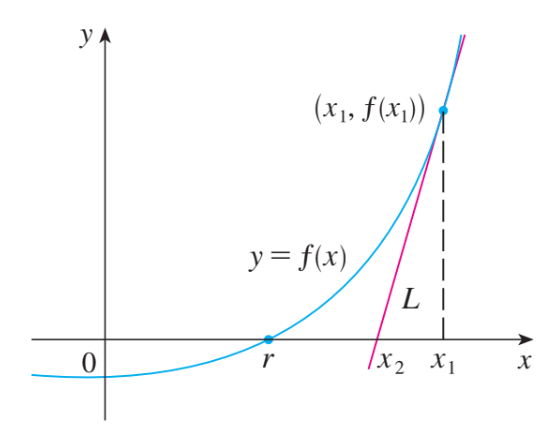
\includegraphics[width=0.4\linewidth]{pic/sec2_1.png}\vspace{0.5cm}\caption{Đồ thị hàm số phi tuyến bất kỳ \cite{stewart2008}} \label{fig:1}\end{figure}\end{center}

\begin{center}\begin{figure}[h]\centering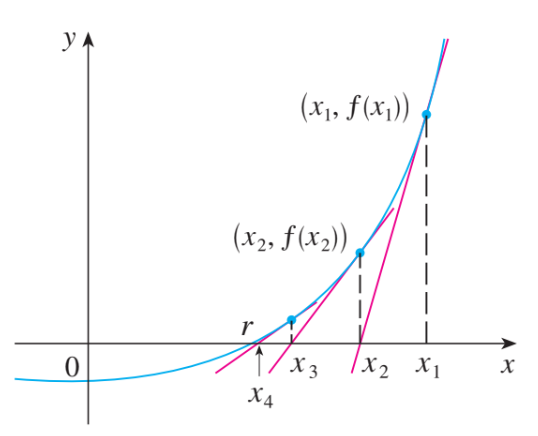
\includegraphics[width=0.4\linewidth]{pic/sec2_2.png}\vspace{0.5cm}\caption{Quá trình hội tụ của nghiệm xấp xỉ qua các bước lặp \cite{stewart2008}}
\label{fig:sec2_2}
\label{fig:2}\end{figure}\end{center}
% 

Để làm cơ sở định lượng chặt chẽ cho trực giác hình học này, ta sử dụng khai triển chuỗi Taylor của hàm $f(x)$ tại lân cận điểm $x_n$:
\begin{equation}
    f(x) \approx f(x_n) + f'(x_n)(x - x_n) + \frac{f''(\xi)}{2!}(x - x_n)^2
    \label{eq:taylor_1d}
\end{equation}
với $\xi$ là một điểm nằm giữa $x$ và $x_n$. Bằng cách tuyến tính hóa hàm số — tức là bỏ qua số hạng bậc hai và các số hạng bậc cao hơn khi $x$ đủ gần $x_n$ — ta thu được biểu thức xấp xỉ tuyến tính (chính là phương trình đường tiếp tuyến $L(x)$):
\begin{equation}
    f(x) \approx L(x) = f(x_n) + f'(x_n)(x - x_n)
\end{equation}
Nghiệm của phương trình phi tuyến $f(x)=0$ lúc này được xấp xỉ bằng nghiệm của phương trình tuyến tính $L(x)=0$. Để tìm điểm xấp xỉ tiếp theo $x_{n+1}$, ta cho $L(x_{n+1}) = 0$:
\begin{equation}
    0 = f(x_n) + f'(x_n)(x_{n+1} - x_n)
\end{equation}
Vì $f'(x_n) \neq 0$, ta chuyển vế và rút ra được \textbf{công thức lặp Newton–Raphson}:
\begin{equation}
    \boxed{x_{n+1} = x_n - \frac{f(x_n)}{f'(x_n)}}, \qquad n = 0, 1, 2, \ldots
    \label{eq:newton_1d}
\end{equation}

Để đảm bảo dãy số $\{x_n\}$ hội tụ về nghiệm $\alpha$, điểm xuất phát $x_0 \in [a,b]$ cần được chọn theo \textbf{điều kiện Fourier}: $f(x_0) \cdot f''(x_0) > 0$ \cite{dau2026hephuongtrinh}.

% Về mặt hình học, phương pháp Newton–Raphson tiếp cận nghiệm bằng cách thay thế đồ thị hàm số $y = f(x)$ bằng tiếp tuyến của nó tại điểm xấp xỉ hiện tại. Để làm cơ sở định lượng chặt chẽ cho trực giác này, ta sử dụng khai triển chuỗi Taylor của hàm $f(x)$ tại lân cận điểm $x_n$:
% \begin{equation}
% f(x) = f(x_n) + f'(x_n)(x - x_n) + \frac{f''(\xi)}{2!}(x - x_n)^2
% \label{eq:taylor_1d}
% \end{equation}
% với $\xi$ là một điểm nằm giữa $x$ và $x_n$. Bằng cách tuyến tính hóa hàm số — tức là bỏ qua số hạng bậc hai và các số hạng bậc cao hơn khi $x$ đủ gần $x_n$ — ta thu được biểu thức xấp xỉ tuyến tính (đường tiếp tuyến):
% \begin{equation}
% f(x) \approx f(x_n) + f'(x_n)(x - x_n)
% \end{equation}
% Để tìm điểm xấp xỉ tiếp theo $x_{n+1}$, ta cho biểu thức xấp xỉ này bằng $0$:
% \begin{equation}
% f(x_n) + f'(x_n)(x_{n+1} - x_n) = 0
% \end{equation}
% Vì $f'(x_n) \neq 0$, ta rút ra được \textbf{công thức lặp Newton–Raphson}:
% \begin{equation}
% \boxed{x_{n+1} = x_n - \frac{f(x_n)}{f'(x_n)}}, \qquad n = 0, 1, 2, \ldots
% \label{eq:newton_formula_1d}
% \end{equation}
% Để đảm bảo dãy số $\{x_n\}$ hội tụ về nghiệm $\alpha$, điểm xuất phát $x_0 \in [a,b]$ cần được chọn theo \textbf{điều kiện Fourier}: $f(x_0) \cdot f''(x_0) > 0$ \cite{dau2026hephuongtrinh}.

% ─────────────────────────────────────────────────────────────
\subsubsection{Phân tích tính hội tụ}



% 


% Trong các phương pháp số, việc một thuật toán tạo ra dãy lặp chưa đủ để đảm bảo tìm được nghiệm đúng. Một thuật toán hiệu quả cần có khả năng hội tụ về nghiệm mong muốn với tốc độ đủ nhanh và ổn định. Cũng như là có thể đánh giá được độ phức tạp của chúng cho việc xem xét tài nguyên sử dụng và thời gian tính toán.

Trước hết ta cần chứng minh dãy $\{x_n\}$ hội tụ nếu ta chọn nghiệm theo điều kiện Fourier. Ta xét 1 đoạn đồ thị trên khoảng phân ly nghiệm $(a,b)$ thì nó sẽ có 4 trường hợp như hình dưới đây 

\begin{figure}[H]
    \centering
    \begin{subfigure}[b]{0.3\textwidth}
        \centering
        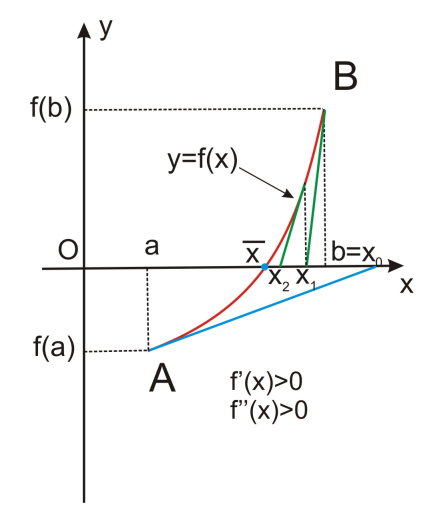
\includegraphics[width=\textwidth]{pic/ppt_sec1_1.png}
        \label{fig:a1}
        \caption{}
    \end{subfigure}
    \hfill
    \begin{subfigure}[b]{0.3\textwidth}
        \centering
        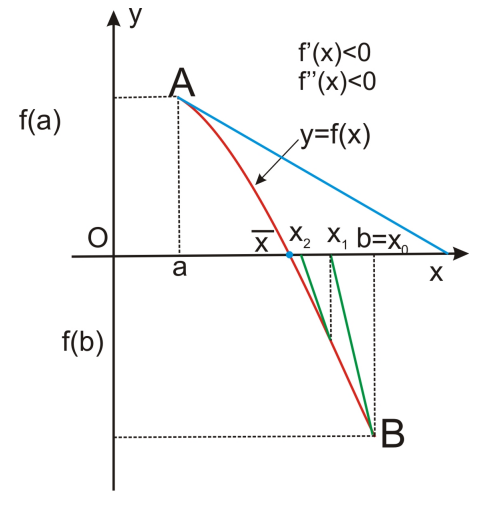
\includegraphics[width=\textwidth]{pic/ppt_sec1_2.png}
        \label{fig:b1}
        \caption{}
    \end{subfigure}
    \hfill
    \begin{subfigure}[b]{0.3\textwidth}
        \centering
        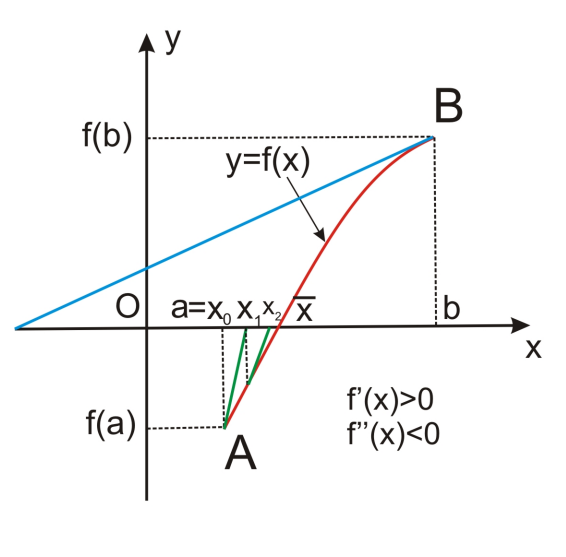
\includegraphics[width=\textwidth]{pic/ppt_sec1_3.png}
        \label{fig:c1}
        \caption{}
    \end{subfigure}
    \hfill
    \begin{subfigure}[b]{0.3\textwidth}
        \centering
        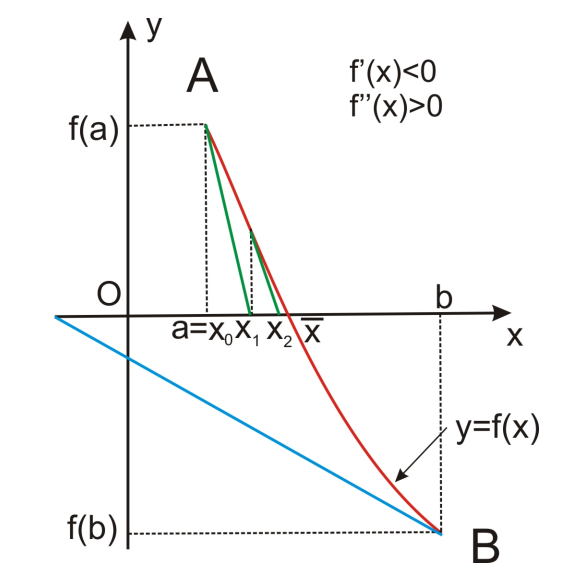
\includegraphics[width=\textwidth]{pic/ppt_sec1_4.png}
        \label{fig:d1}
        \caption{}
    \end{subfigure}
    
    \caption{Các trường hợp xảy ra Nguồn: \cite{dau2026hephuongtrinh}}
    \label{fig:ba-hinh}
\end{figure}

Xét hình (a) và (b) ta được 
$$a < \bar{x} < \dots < x_n < x_{n-1} < \dots < x_1 < x_0 = b$$

Và hình (c) và (d) sẽ cho ta được kết quả 

$$a = x_0 < x_1 < \dots < x_{n-1} < x_n < \dots < \bar{x} < b$$

Do đó với các trường hợp có thể của đồ thị thì thấy dãy đơn điệu và bị chặn. Do đó ta có được dãy hội tụ theo định lý Weierstrass.

% Độ hội tụ của một thuật toán lặp mô tả khả năng mà dãy nghiệm gần đúng sinh ra bởi thuật toán tiến dần đến nghiệm chính xác của bài toán. 

% Giả sử $\alpha$ là nghiệm đúng của hệ phương trình và $x_n$ là nghiệm gần đúng tại bước lặp thứ $n$, ta định nghĩa sai số tại bước lặp thứ $n$ là
% \[
% e_n = \|x_n-\alpha\|.
% \]

% Một thuật toán được gọi là hội tụ nếu
% \[
% \lim_{n\to\infty} e_n = 0.
% \]

% Ngoài việc xét thuật toán có hội tụ hay không, tốc độ giảm của sai số cũng là một yếu tố quan trọng. Trong phân tích số, tốc độ hội tụ thường được mô tả thông qua cấp hội tụ (order of convergence), được xác định bởi quan hệ
% \[
% e_{n+1}\approx Ce_n^p,
% \]
% với $C>0$ và $p$ được gọi là cấp hội tụ của thuật toán.

% Nếu $p=1$ thì hệ hội tụ tuyến tính, còn nếu $p=2$ thì thuật toán có hội tụ bậc hai. Phương pháp Newton là một ví dụ tiêu biểu của thuật toán có hội tụ bậc hai khi giá trị khởi tạo đủ gần nghiệm đúng.

% \textbf{Chứng minh ~\cite{chapra_ch6}:}
% Ta gọi $\alpha$ là nghiệm chính xác, tức $f(\alpha) = 0$. Tại bước lặp thứ $n$. Khi đó ta có sai số tại $n$ 

% \begin{equation}
%     e_n = x_n - \alpha \quad \implies \quad \alpha = x_n - e_n.
%     \label{eq:error_def}
% \end{equation}


% Khai triển Taylor của $f$ tại $x_n$, đánh giá tại $\alpha$ và dùng $f(\alpha) = 0$:

% \begin{equation}
%     0 = f(x_n) + f'(x_n)\,(\alpha - x_n) + \frac{f''(\xi)}{2}\,(\alpha - x_n)^2,
%     \label{eq:conv_taylor}
% \end{equation}

% trong đó $\xi$ nằm giữa $x_n$ và $\alpha$. Thay $\alpha - x_n = -e_n$:

% \begin{equation}
%     0 = f(x_n) - e_n f'(x_n) + \frac{e_n^2}{2}\, f''(\xi).
%     \label{eq:conv_taylor2}
% \end{equation}

% Chia cho $f'(x_n) \neq 0$:

% \begin{equation}
%     0 = \frac{f(x_n)}{f'(x_n)} - e_n + \frac{f''(\xi)}{2f'(x_n)}\, e_n^2.
%     \label{eq:conv_div}
% \end{equation}

% Từ công thức lặp \eqref{eq:newton_1d}, trừ cả hai vế cho $\alpha$:

% \begin{equation}
%     e_{n+1} = x_{n+1} - \alpha = e_n - \frac{f(x_n)}{f'(x_n)}.
%     \label{eq:error_recur}
% \end{equation}

% Kết hợp \eqref{eq:conv_div} và \eqref{eq:error_recur}:

% \begin{equation}
%     \boxed{e_{n+1} = \frac{f''(\xi)}{2\,f'(x_n)}\, e_n^2.}
%     \label{eq:quadratic_convergence}
% \end{equation}

% Hệ thức chứng minh \textbf{tính hội tụ bậc hai} của phương pháp Newton–Raphson: sai số ở bước tiếp theo tỷ lệ với \textit{bình phương} sai số hiện tại. Nếu $|e_n| \approx 10^{-2}$, thì $|e_{n+1}| \approx 10^{-4}$, rồi $10^{-8}$, v.v.

Để đánh giá tốc độ giảm của sai số, trong phân tích số người ta thường sử dụng khái niệm \textit{cấp hội tụ} (order of convergence). Gọi sai số tại bước lặp thứ $n$ là $e_n = x_n - \alpha$. Nếu tồn tại hằng số $C > 0$ và số thực $p \ge 1$ sao cho:
\begin{equation}
    |e_{n+1}| \approx C |e_n|^p
\end{equation}
thì $p$ được gọi là cấp hội tụ. Với phương pháp Newton–Raphson 1 ẩn, ta sẽ chứng minh thuật toán đạt cấp hội tụ $p = 2$ (hội tụ bậc hai) khi điểm khởi tạo đủ gần nghiệm \cite{chapra_ch6}.

\textbf{Chứng minh:}
Ta có nghiệm chính xác là $\alpha$, tức $f(\alpha) = 0$. Sai số tại bước lặp thứ $n$ được xác định bởi:
\begin{equation}
    e_n = x_n - \alpha \quad \implies \quad \alpha = x_n - e_n.
    \label{eq:error_def}
\end{equation}
Khai triển chuỗi Taylor của hàm số $f$ tại lân cận $x_n$, đánh giá tại điểm $\alpha$ và kết hợp điều kiện $f(\alpha) = 0$, ta có:
\begin{equation}
    0 = f(\alpha) = f(x_n) + f'(x_n)\,(\alpha - x_n) + \frac{f''(\xi)}{2}\,(\alpha - x_n)^2,
    \label{eq:conv_taylor}
\end{equation}
trong đó $\xi$ là một điểm nằm giữa $x_n$ và $\alpha$. Thay $\alpha - x_n = -e_n$ vào \eqref{eq:conv_taylor}:
\begin{equation}
    0 = f(x_n) - e_n f'(x_n) + \frac{e_n^2}{2}\, f''(\xi).
    \label{eq:conv_taylor2}
\end{equation}
Chia cả hai vế cho $f'(x_n) \neq 0$:
\begin{equation}
    0 = \frac{f(x_n)}{f'(x_n)} - e_n + \frac{f''(\xi)}{2f'(x_n)}\, e_n^2.
    \label{eq:conv_div}
\end{equation}
Mặt khác, từ công thức lặp Newton–Raphson \eqref{eq:newton_1d}, trừ cả hai vế cho $\alpha$ để thiết lập hệ thức truy hồi cho sai số:
\begin{equation}
    x_{n+1} - \alpha = x_n - \alpha - \frac{f(x_n)}{f'(x_n)} \quad \implies \quad e_{n+1} = e_n - \frac{f(x_n)}{f'(x_n)}.
    \label{eq:error_recur}
\end{equation}
Từ \eqref{eq:error_recur}, ta suy ra $e_n - e_{n+1} = \frac{f(x_n)}{f'(x_n)}$. Thay thế đại lượng này vào phương trình \eqref{eq:conv_div}, ta thu được:
\begin{equation}
    \boxed{e_{n+1} = \frac{f''(\xi)}{2\,f'(x_n)}\, e_n^2.}
    \label{eq:quadratic_convergence}
\end{equation}

\textbf{Kết luận:} Hệ thức \eqref{eq:quadratic_convergence} chứng minh rõ ràng tính hội tụ bậc hai của phương pháp Newton–Raphson, vì sai số ở bước lặp tiếp theo tỷ lệ thuận với bình phương sai số của bước trước đó. Nếu tại một bước lặp sai số đạt $|e_n| \approx 10^{-2}$, thì ở các bước tiếp theo sai số sẽ giảm cực nhanh theo cấp số mũ: $|e_{n+1}| \approx 10^{-4}$, rồi $10^{-8}$, $10^{-16}$, v.v.

\begin{bt}{Ví dụ}
    Cho phương trình $f(x) = x^3 - 3x + 1$ trong khoảng cách ly nghiệm $[0;\, 0{,}5]$. Tìm nghiệm gần đúng $x_3$ bằng phương pháp Newton–Raphson.
\end{bt}
\noindent{\textbf{Giải.}}

Ta có $f(0) > 0$, $f(0{,}5) < 0$, $f'(x) = 3x^2 - 3 < 0$ với mọi $x\in[0;\,0{,}5]$, và $f''(x) = 6x \geq 0$ với mọi $x\in[0;\,0{,}5]$, nên theo điều kiện Fourier ta chọn $x_0 = 0$.

Áp dụng công thức lặp \eqref{eq:newton_1d}:

\begin{equation}
    x_n = x_{n-1} - \frac{f(x_{n-1})}{f'(x_{n-1})}
        = x_{n-1} - \frac{x_{n-1}^3 - 3x_{n-1} + 1}{3x_{n-1}^2 - 3}
        = \frac{2x_{n-1}^3 - 1}{3x_{n-1}^2 - 3}.
    \label{eq:example_iter}
\end{equation}

\begin{table}[h]
\centering
\begin{tabular}{|c|c|c|}
\hline
$n$ & $x_n$ & $\Delta x_n = |x_n - x_{n-1}|$ \\
\hline
1 & 0.3333333333 & 3.33333333e-01 \\
\hline
2 & 0.3472222222 &1.38888889e-02 \\
\hline
3 & 0.3472963532 &7.41309416e-05\\
\hline
4 & 0.3472963553 &2.16999265e-09\\
\hline
\end{tabular}
\end{table}


\subsection{ Mở rộng cho hệ phương trình phi tuyến $n$ biến}

Một câu hỏi quan trọng được đặt ra: Làm thế nào để giải quyết các bài toán thực tế khi không chỉ có một biến số mà là một hệ gồm $n$ phương trình với $n$ ẩn số?

Về mặt trực giác, nếu ở không gian $Oxy$ ta dùng \textbf{đường tiếp tuyến} để xấp xỉ đường cong, thì ở không gian nhiều 3 chiều ta sẽ dùng các \textbf{mặt phẳng tiếp diện} để xấp xỉ các mặt cong phức tạp tại điểm dự đoán ban đầu.

% ─────────────────────────────────────────────────────────────

\subsubsection{Nội dung phương pháp cho $n$ chiều}

Xét hệ $n$ phương trình $n$ biến:

\begin{equation}
    \begin{cases}
        f_1(x_1, x_2, \dots, x_n) = 0, \\
        f_2(x_1, x_2, \dots, x_n) = 0, \\
        \quad \vdots \\
        f_n(x_1, x_2, \dots, x_n) = 0.
    \end{cases}
    \label{eq:system}
\end{equation}

Giả sử các hàm $f_i$ ($i = \overline{1,n}$) và các đạo hàm riêng của chúng đến bậc hai đều liên tục và tồn tại. Khai triển Taylor bậc nhất của $f_i$ tại lân cận điểm $(x_1,\dots,x_n)$:

\begin{equation}
   f_i(x_1 +h_1,\dots,x_n+h_n) \approx f_i(x_1,\dots,x_n) + h_1\dfrac{\partial f_i (x_1,\dots,x_n)}{\partial x_1} + \dots + h_n\dfrac{\partial f_i (x_1,\dots,x_n)}{\partial x_n}
   \label{eq:taylor_system}
\end{equation}

Gộp $n$ khai triển \eqref{eq:taylor_system} lại, ta được hệ phương trình:
\begin{equation}
\begin{cases}
 f_1(x_1 +h_1,\dots,x_n+h_n) \approx f_1(x_1,\dots,x_n) + h_1\dfrac{\partial f_1 (x_1,\dots,x_n)}{\partial x_1} + \dots + h_n\dfrac{\partial f_1 (x_1,\dots,x_n)}{\partial x_n} \\
 f_2(x_1 +h_1,\dots,x_n+h_n) \approx f_2(x_1,\dots,x_n) + h_1\dfrac{\partial f_2 (x_1,\dots,x_n)}{\partial x_1} + \dots + h_n\dfrac{\partial f_2 (x_1,\dots,x_n)}{\partial x_n} \\
 \quad \vdots \\
 f_n(x_1 +h_1,\dots,x_n+h_n) \approx f_n(x_1,\dots,x_n) + h_1\dfrac{\partial f_n (x_1,\dots,x_n)}{\partial x_1} + \dots + h_n\dfrac{\partial f_n (x_1,\dots,x_n)}{\partial x_n}
\end{cases}
\label{eq:linear_system}
\end{equation}

Ta đặt vector trạng thái hiện tại là $\mathbf{x}^{(0)} = (x_1,\dots,x_n)^\top$, vector trạng thái mới là $\mathbf{x}^{(1)} = (x_1+h_1,\dots,x_n+h_n)^\top$, và vector bước lặp là $\mathbf{h} = (h_1, h_2, \dots, h_n)^\top$. 

Hệ \eqref{eq:linear_system} có thể được viết gọn lại dưới dạng ma trận:

\begin{equation}
    \mathbf{F}(\mathbf{x}^{(1)}) \approx \mathbf{F}(\mathbf{x}^{(0)}) + \mathbf{J}(\mathbf{x}^{(0)}) \mathbf{h}
    \label{eq:matrix_form}
\end{equation}

Trong đó, $\mathbf{F}(\mathbf{x})$ là vector chứa các hàm $f_i$, và $\mathbf{J}(\mathbf{x}^{(0)})$ là \textbf{ma trận Jacobian} cấp $n \times n$ được định nghĩa như sau:
\begin{equation}
    \mathbf{J}(\mathbf{x}^{(0)}) =
    \begin{pmatrix}
        \dfrac{\partial f_1}{\partial x_1} & \dfrac{\partial f_1}{\partial x_2} & \cdots & \dfrac{\partial f_1}{\partial x_n} \\[8pt]
        \dfrac{\partial f_2}{\partial x_1} & \dfrac{\partial f_2}{\partial x_2} & \cdots & \dfrac{\partial f_2}{\partial x_n} \\[4pt]
        \vdots & \vdots & \ddots & \vdots \\[4pt]
        \dfrac{\partial f_n}{\partial x_1} & \dfrac{\partial f_n}{\partial x_2} & \cdots & \dfrac{\partial f_n}{\partial x_n}
    \end{pmatrix}_{\!\mathbf{x} = \mathbf{x}^{(0)}}
    \label{eq:jacobian_def}
\end{equation}

Xét cho $\mathbf{F}(\mathbf{x}^{(1)}) = \mathbf{0}$ khi đó ta được $\mathbf{h = x^{(1)} - x^{(0)}} $

Thay vào phương trình \eqref{eq:matrix_form}, ta có:
\begin{equation}
    \mathbf{0} \approx \mathbf{F}(\mathbf{x}^{(0)}) + \mathbf{J}(\mathbf{x}^{(0)}) \mathbf{h}
\end{equation}

Chuyển vế, ta thu được hệ phương trình đại số tuyến tính đối với vector ẩn $\mathbf{h}$:
\begin{equation}
    \mathbf{J}(\mathbf{x}^{(0)}) \mathbf{h} = -\mathbf{F}(\mathbf{x}^{(0)})
    \label{eq:solve_h}
\end{equation}

Giả sử ma trận Jacobian $\mathbf{J}(\mathbf{x}^{(0)})$ không suy biến (tức là $\det(\mathbf{J}) \neq 0$), ta có thể tìm được $\mathbf{h}$ bằng cách nhân cả hai vế với ma trận nghịch đảo $\mathbf{J}^{-1}(\mathbf{x}^{(0)})$:
\begin{equation}
    \mathbf{h} = -[\mathbf{J}(\mathbf{x}^{(0)})]^{-1} \mathbf{F}(\mathbf{x}^{(0)})
\end{equation}

Vì $\mathbf{x}^{(1)} = \mathbf{x}^{(0)} + \mathbf{h}$, ta suy ra trạng thái ở bước tiếp theo:
\begin{equation}
    \mathbf{x}^{(1)} = \mathbf{x}^{(0)} - [\mathbf{J}(\mathbf{x}^{(0)})]^{-1} \mathbf{F}(\mathbf{x}^{(0)})
\end{equation}

Khái quát hóa quá trình này cho bước lặp thứ $k$ (với $k = 0, 1, 2, \dots$), ta nhận được \textbf{công thức lặp Newton-Raphson} dạng tổng quát:
\begin{equation}
    \mathbf{x}^{(k+1)} = \mathbf{x}^{(k)} - [\mathbf{J}(\mathbf{x}^{(k)})]^{-1} \mathbf{F}(\mathbf{x}^{(k)})
    \label{eq:newton_raphson_general}
\end{equation}

% Xét hệ $n$ phương trình $n$ biến:

% \begin{equation}
%     \begin{cases}
%         f_1(x_1, x_2, \dots, x_n) = 0, \\
%         f_2(x_1, x_2, \dots, x_n) = 0, \\
%         \quad \vdots \\
%         f_n(x_1, x_2, \dots, x_n) = 0.
%     \end{cases}
%     \label{eq:system}
% \end{equation}

% Giả sử các hàm $f_i$ ($i = \overline{1,n}$) và các đạo hàm riêng của chúng đến bậc hai đều liên tục và tồn tại. Khai triển Taylor của $f_i$ tại lân cận điểm $(x_1,\dots,x_n)$ 

% \begin{equation}
%    f_i(x_1 +h_1,\dots,x_n+h_n) = f_i(x_1,\dots,x_n)+h_1.\dfrac{\partial f_i (x_1,\dots,x_n)}{x_1} +...+h_n. \dfrac{\partial f_i (x_1,\dots,x_n)}{x_n}
%    \label{eq:taylor_system}
% \end{equation}

% Gộp $n$ hệ \eqref{eq:taylor_system}  lại ta viết thành dạng ma trận:
% \begin{equation}
% \begin{cases}
%  f_1(x_1 +h_1,\dots,x_n+h_n) = f_1(x_1,\dots,x_n)+h_1.\dfrac{\partial f_1 (x_1,\dots,x_n)}{\partial x_1} +...+h_n. \dfrac{\partial f_1 (x_1,\dots,x_n)}{\partial x_n}\\
%   f_2(x_1 +h_1,\dots,x_n+h_n) = f_2(x_1,\dots,x_n)+h_1.\dfrac{\partial f_2 (x_1,\dots,x_n)}{\partial x_1} +...+h_n. \dfrac{\partial f_2 (x_1,\dots,x_n)}{\partial x_n} \\
%   \dots \\
%    f_n(x_1 +h_1,\dots,x_n+h_n) = f_n(x_1,\dots,x_n)+h_1.\dfrac{\partial f_n (x_1,\dots,x_n)}{\partial x_1} +...+h_n. \dfrac{\partial f_n (x_1,\dots,x_n)}{\partial x_n}
    
%     \label{eq:linear_system}
% \end{cases}
% \end{equation}

% Ta đặt $\mathbf{x^{(0)}}= (x_1,\dots,x_n)$ và $\mathbf{x^{(1)}}= (x_1+h_1,\dots,x_n+h_n)$.

% Hay viết gọn dưới dạng vector: $\mathbf{F}(\mathbf{x^{(0)}}) = \begin{bmatrix}
%     f_1(x_1,\dots,x_n)\\
%     f_2(x_1,\dots,x_n)\\
%     \vdots \\
%     f_n(x_1,\dots,x_n)
% \end{bmatrix} $. Ta rút gọn hệ \ref{eq:linear_system} lại thành các ma trận nhân nhau và với ẩn $\mathbf{h} = (h_1, h_2, \dots, h_n)^\top$ ta được

% \begin{equation}
%     \mathbf{F(x^{(1)})} = \mathbf{F(x^{(0)})} +\mathbf{J}(\mathbf{x}^{(0)}).\mathbf{h}
% \end{equation}


% trong đó $\mathbf{J}(\mathbf{x}^{(0)})$ là \textbf{ma trận Jacobian} cấp $n\times n$:
% \begin{equation}
%     \mathbf{J}(\mathbf{x}^{(0)}) =
%     \begin{pmatrix}
%         \dfrac{\partial f_1}{\partial x_1} & \dfrac{\partial f_1}{\partial x_2} & \cdots & \dfrac{\partial f_1}{\partial x_n} \\[8pt]
%         \dfrac{\partial f_2}{\partial x_1} & \dfrac{\partial f_2}{\partial x_2} & \cdots & \dfrac{\partial f_2}{\partial x_n} \\[4pt]
%         \vdots & \vdots & \ddots & \vdots \\[4pt]
%         \dfrac{\partial f_n}{\partial x_1} & \dfrac{\partial f_n}{\partial x_2} & \cdots & \dfrac{\partial f_n}{\partial x_n}
%     \end{pmatrix}_{\!\mathbf{x} = \mathbf{x}^{(0)}}.
%     \label{eq:jacobian_def}
% \end{equation}

Nếu $\mathbf{J}(\mathbf{x}^{(0)})$ khả nghịch, nghiệm của \eqref{eq:linear_system} là:

\begin{equation}
    \mathbf{h} = -\mathbf{J}^{-1}\!\left(\mathbf{x}^{(0)}\right)\, \mathbf{F}\!\left(\mathbf{x}^{(0)}\right).
    \label{eq:h_solution}
\end{equation}

Do đó, điểm xấp xỉ tiếp theo là:

\begin{equation}
    \mathbf{x}^{(k+1)} = \mathbf{x}^{(k)} - \mathbf{J}^{-1}\!\left(\mathbf{x}^{(k)}\right)\, \mathbf{F}\!\left(\mathbf{x}^{(k)}\right), \qquad k = 0,1,2,\ldots
    \label{eq:newton_nd}
\end{equation}

Quá trình lặp lại: tính $\mathbf{J}(\mathbf{x}^{(k+1)})$ và tiếp tục cho đến khi $\mathbf{x}$ hội tụ.

Thay vì tìm giao điểm của các mặt cong phi tuyến phức tạp, thuật toán liên tục xấp xỉ chúng bằng các mặt phẳng tiếp tuyến — một bài toán tuyến tính đơn giản hơn nhiều.

Khi này ta có phát biểu tổng quát hơn và chặt chẽ hơn.


\begin{bt}{Phương pháp Newton cho hệ phương trình phi tuyến}
Xét hệ phương trình phi tuyến:
$$
\mathbf{F}(\mathbf{x})=\mathbf{0}
$$
với $\mathbf{F}: D \subset \mathbb{R}^n \rightarrow \mathbb{R}^n$, trong đó $D$ là một tập mở.

Giả sử $\mathbf{F}$ là hàm khả vi liên tục trên $D$ và ma trận Jacobian $\mathbf{J}\!\left(\mathbf{x}^{(k)}\right)$ không suy biến (khả nghịch) tại mọi bước lặp $k$. 
Bắt đầu từ vector khởi tạo $\mathbf{x}^{(0)} \in D$, giả sử mọi xấp xỉ $\mathbf{x}^{(k)}$ đều thuộc $D$, dãy lặp Newton được xác định bởi công thức:
\begin{equation}
    \mathbf{x}^{(k+1)}
    =
    \mathbf{x}^{(k)}
    -
    \mathbf{J}^{-1}\!\left(\mathbf{x}^{(k)}\right)\mathbf{F}\!\left(\mathbf{x}^{(k)}\right), \quad k = 0, 1, 2, \dots
\end{equation}
\end{bt}

% \begin{bt}{Ví dụ}
%      Cho hệ phương trình:
% $$
% \begin{cases} 
% u(x, y) = x^2 + xy - 10 = 0 \\ 
% v(x, y) = y + 3xy^2 - 57 = 0 
% \end{cases} 
% $$
% cho biết nghiệm chính xác $(x = 2, y = 3)$.\\
% Nghiệm ban đầu cho $(x_0 = 1{,}5; y_0 = 3{,}5)$.

% \end{bt}
% \textbf{Giải}

% Ta tính các đạo hàm riêng (các phần tử của ma trận Jacobian):
% $$
% \begin{aligned}
% \frac{\partial v}{\partial y} &= 1 + 6xy &\implies \frac{\partial v_0}{\partial y_0} &= 1 + 6(1{,}5)(3{,}5) = 32{,}5 \\
% \frac{\partial v}{\partial x} &= 3y^2 &\implies \frac{\partial v_0}{\partial x_0} &= 3(3{,}5)^2 = 36{,}75 \\
% \frac{\partial u}{\partial y} &= x &\implies \frac{\partial u_0}{\partial y_0} &= 1{,}5 \\
% \frac{\partial u}{\partial x} &= 2x + y &\implies \frac{\partial u_0}{\partial x_0} &= 2(1{,}5) + 3{,}5 = 6{,}5
% \end{aligned}
% $$

% Định thức Jacobian: 
% $$ 
% \det J_0 = \frac{\partial u_0}{\partial x_0}\frac{\partial v_0}{\partial y_0} - \frac{\partial u_0}{\partial y_0}\frac{\partial v_0}{\partial x_0} = 6{,}5(32{,}5) - 1{,}5(36{,}75) = 156{,}125 
% $$

% Giá trị các hàm tại điểm ban đầu $(x_0, y_0)$:
% $$
% \begin{aligned}
% u_0 &= (1{,}5)^2 + 1{,}5(3{,}5) - 10 = -2{,}5 \\
% v_0 &= 3{,}5 + 3(1{,}5)(3{,}5)^2 - 57 = 1{,}625
% \end{aligned}
% $$

% Áp dụng công thức Newton-Raphson cho hệ phương trình, ta có bước 1 ($n=1$):
% $$
% \begin{cases}
% x_1 = x_0 - \dfrac{u_0 \frac{\partial v_0}{\partial y_0} - v_0 \frac{\partial u_0}{\partial y_0}}{\det J_0} = 1{,}5 - \dfrac{-2{,}5(32{,}5) - 1{,}625(1{,}5)}{156{,}125} \approx 2{,}03603 \\[15pt]
% y_1 = y_0 - \dfrac{v_0 \frac{\partial u_0}{\partial x_0} - u_0 \frac{\partial v_0}{\partial x_0}}{\det J_0} = 3{,}5 - \dfrac{1{,}625(6{,}5) - (-2{,}5)(36{,}75)}{156{,}125} \approx 2{,}84388
% \end{cases}
% $$

% Tiếp tục các bước xấp xỉ tương tự, nghiệm sẽ dần hội tụ về $(x = 2, y = 3)$.

% \vspace{1cm}
% \textbf{Bảng tổng hợp kết quả các bước lặp:}
% \vspace{0.3cm}

% \begin{center}
% \renewcommand{\arraystretch}{1.5}
% \begin{tabular}{|c|c|c|c|c|c|c|}
% \hline
% $n$ & $x_n$ & $y_n$ & $u(x_n, y_n)$ & $v(x_n, y_n)$ & $\Delta x_n = |x_n - x_{n-1}|$ & $\Delta y_n = |y_n - y_{n-1}|$ \\
% \hline
% 0 & $1{,}50000$ & $3{,}50000$ & $-2{,}50000$ & $1{,}62500$ & --- & --- \\
% \hline
% 1 & $2{,}03603$ & $2{,}84388$ & $-0{,}06437$ & $-4{,}75621$ & $0{,}53603$ & $0{,}65612$ \\
% \hline
% 2 & $1{,}99870$ & $3{,}00229$ & $-0{,}00452$ & $0{,}04957$ & $0{,}03733$ & $0{,}15841$ \\
% \hline
% 3 & $2{,}00000$ & $3{,}00000$ & $0{,}00000$ & $0{,}00000$ & $0{,}00130$ & $0{,}00229$ \\
% \hline
% \end{tabular}
% \end{center}
% ─────────────────── ──────────────────────────────────────────
% \subsection{Ma trận Jacobian}

% \begin{itemize}
%     \item Ma trận Jacobian là công cụ cốt lõi trong giải tích nhiều biến và giải tích vector.
%     \item Khi chuyển từ hàm một biến sang hàm vector nhiều biến, khái niệm đạo hàm cần được mở rộng để phản ánh sự thay đổi đồng thời của nhiều thành phần.
%     \item Ma trận Jacobian chính là sự tổng quát hóa của đạo hàm . Ý nghĩa hình học của nó là dùng một ma trận để xấp xỉ tuyến tính hàm số tại một điểm 
% \end{itemize}

% \textbf{a) Định nghĩa.~\cite{wikipedia_jacobian}}

% Cho $\mathbf{f} : \mathbb{R}^n \to \mathbb{R}^m$ sao cho mỗi đạo hàm riêng bậc nhất tồn tại trên $\mathbb{R}^n$. Hàm nhận $\mathbf{x} = (x_1,\dots,x_n)^\top \in \mathbb{R}^n$ và trả về $\mathbf{f}(\mathbf{x}) = (f_1(\mathbf{x}),\dots,f_m(\mathbf{x}))^\top \in \mathbb{R}^m$. Ma trận Jacobian $\mathbf{J}_{\mathbf{f}}$ là ma trận cấp $m \times n$ chứa tất cả đạo hàm riêng của hàm số :

% \begin{equation}
%     \mathbf{J}_{\mathbf{f}} =
%     \begin{bmatrix}
%         \nabla^\top f_1 \\ \vdots \\ \nabla^\top f_m
%     \end{bmatrix}
%     =
%     \begin{bmatrix}
%         \dfrac{\partial f_1}{\partial x_1} & \cdots & \dfrac{\partial f_1}{\partial x_n} \\[8pt]
%         \vdots & \ddots & \vdots \\[4pt]
%         \dfrac{\partial f_m}{\partial x_1} & \cdots & \dfrac{\partial f_m}{\partial x_n}
%     \end{bmatrix},
%     \label{eq:jacobian_full}
% \end{equation}

% trong đó $\nabla^\top f_i$ là gradient hàng (chuyển vị của gradient) của thành phần $f_i$.

% \textbf{Ví dụ 1.~\cite{wikipedia_jacobian}} Xét $\mathbf{F} : \mathbb{R}^2 \to \mathbb{R}^3$ với
% \begin{equation}
%     \mathbf{F}(x, y) =
%     \begin{bmatrix} x^2 y \\ 5x + \sin y \\ 4y \end{bmatrix}.
%     \label{eq:example_f}
% \end{equation}
% Ma trận Jacobian của $\mathbf{F}$:
% \begin{equation}
%     \mathbf{J}_{\mathbf{F}}(x,y) =
%     \begin{bmatrix}
%         2xy  & x^2 \\
%         5    & \cos y \\
%         0    & 4
%     \end{bmatrix}.
%     \label{eq:example_J}
% \end{equation}

% \textbf{b) Ý nghĩa hình học và xấp xỉ tuyến tính. ~\cite{wikipedia_jacobian}}

% Giả sử $\mathbf{F} : \mathbb{R}^n \to \mathbb{R}^m$ khả vi tại $\mathbf{p}$. Phép xấp xỉ tuyến tính tốt nhất của $\mathbf{f}$ trong lân cận $\mathbf{p}$:

% \begin{equation}
%     \mathbf{F}(\mathbf{x}) = \mathbf{F}(\mathbf{p}) + \mathbf{J}_{\mathbf{F}}(\mathbf{p})\,(\mathbf{x} - \mathbf{p}) + o\!\left(\|\mathbf{x}-\mathbf{p}\|\right)
%     \label{eq:linear_approx_nd}
% \end{equation}

% Đối với hàm một biến $f:\mathbb{R}\to\mathbb{R}$, \eqref{eq:linear_approx_nd} thu gọn về đa thức Taylor bậc nhất (phương trình tiếp tuyến):
% \begin{equation}
%     f(x) = f(p) + f'(p)\,(x-p) + o(x-p).
%     \label{eq:taylor_1d_approx}
% \end{equation}

% \begin{itemize}
%     \item Trong không gian 1 chiều: $f'(p)$ là hệ số góc của đường tiếp tuyến tại điểm $p$ tạo ra \textbf{đường thẳng tiếp tuyến}.
%     \item Trong không gian $n$ chiều: $\mathbf{J}_{\mathbf{f}}(\mathbf{p})$ cũng tương tự nhưng sẽ là gradient của hàm số và tạo ra \textbf{không gian tiếp xúc} (mặt phẳng tiếp diện).
% \end{itemize}

% \textbf{Ví dụ 2.} Xét $\mathbf{F}(x,y) = \begin{bmatrix} x^2+y \\ 2xy \end{bmatrix}$.
% Ma trận Jacobian:
% \begin{equation}
%     \mathbf{J}(x,y) =
%     \begin{bmatrix} 2x & 1 \\ 2y & 2x \end{bmatrix};
%     \qquad
%     \mathbf{J}(1,1) =
%     \begin{bmatrix} 2 & 1 \\ 2 & 2 \end{bmatrix}.
%     \label{eq:jacobian_example2}
% \end{equation}

% Tại $(x_0,y_0) = (1,1)$: $\mathbf{F}(1,1) = \begin{bmatrix} 2 \\ 2 \end{bmatrix}$.

% Xấp xỉ tuyến tính tại $\Delta\mathbf{x} = (0{,}1,\,-0{,}1)^\top$:
% \begin{equation}
%     \mathbf{F}(1{,}1;\,0{,}9) \approx \mathbf{F}(1,1) + \mathbf{J}(1,1)\,\Delta\mathbf{x}
%     = \begin{bmatrix}2\\2\end{bmatrix} + \begin{bmatrix}2&1\\2&2\end{bmatrix}\begin{bmatrix}0{,}1\\-0{,}1\end{bmatrix}
%     = \begin{bmatrix}2{,}1\\2\end{bmatrix}.
%     \label{eq:linearization_example}
% \end{equation}

% Giá trị thực: $f_1(1{,}1;\,0{,}9) = 2{,}11$; $f_2(1{,}1;\,0{,}9) = 1{,}98$. Kết quả xấp xỉ rất sát, minh chứng sức mạnh của phép tuyến tính hóa.

% % ─────────────────────────────────────────────────────────────
% \subsubsection{ Phân tích tính hội tụ của thuật toán }

\subsubsection{Đánh giá sai số và điều kiện dừng}Trong phương pháp Newton không gian một chiều, sai số xấp xỉ giữa hai bước lặp liên tiếp được xác định đơn giản thông qua giá trị tuyệt đối của khoảng cách:\begin{equation}\Delta x = \left| x^{(k)} - x^{(k-1)} \right|\end{equation}Tuy nhiên, đối với hệ phương trình đa biến, nghiệm xấp xỉ tại mỗi bước lặp là các vector $\mathbf{x}^{(k)}$. Việc đánh giá sai số lúc này không thể chỉ dựa trên phép trừ vector đơn thuần, mà đòi hỏi việc sử dụng các \textbf{chuẩn (norms)} trong không gian vector để ánh xạ toàn bộ sai số của hệ thống thành một đại lượng vô hướng duy nhất.Gọi vector nghiệm tại bước lặp thứ $k$ là $\mathbf{x}^{(k)}$ và bước trước đó là $\mathbf{x}^{(k-1)}$. Vector sai số bước lặp được định nghĩa là:\begin{equation}\Delta\mathbf{x} = \mathbf{x}^{(k)} - \mathbf{x}^{(k-1)}\end{equation}Trong thực hành tính toán số, hai loại chuẩn sau đây thường được áp dụng phổ biến nhất để thiết lập tiêu chuẩn hội tụ (điều kiện dừng) cho thuật toán:\begin{itemize}\item \textbf{Chuẩn 1 (Norm 1) — Tổng sai số tuyệt đối:}Chuẩn 1 đánh giá tổng mức độ sai lệch của toàn bộ hệ thống bằng cách lấy tổng giá trị tuyệt đối các thành phần của vector sai số:\begin{equation}|| \Delta\mathbf{x} ||_ 1 = \sum_{i=1}^{n} \left| x_i^{(k)} - x_i^{(k-1)} \right|\end{equation}Tiêu chuẩn này thường được sử dụng khi các biến trong hệ phương trình có vai trò ngang hàng và ta quan tâm đến sự hội tụ tích lũy của toàn hệ thống.\item \textbf{Chuẩn vô cùng (Infinity Norm) — Sai số cực đại:}
Chuẩn vô cùng đánh giá sai số dựa trên thành phần có sự sai lệch lớn nhất trong vector:
\begin{equation}
    \| \Delta\mathbf{x} \|_\infty = \max_{1 \le i \le n} \left| x_i^{(k)} - x_i^{(k-1)} \right|
\end{equation}
Đây là điều kiện dừng an toàn và khắt khe nhất. Nếu ta thiết lập ngưỡng dung sai $\| \Delta\mathbf{x} \|_\infty < \varepsilon$ (ví dụ $\varepsilon = 10^{-4}$), điều này đảm bảo chắc chắn rằng \textit{không có bất kỳ một biến đơn lẻ nào} trong hệ có sai số vượt qua ngưỡng cho phép. Trong mô phỏng kỹ thuật, chuẩn vô cùng thường được ưu tiên để tránh hiện tượng hội tụ giả.
\end{itemize}

% \subsubsection{Độ phức tạp thuật toán}
% Trong tính toán số, \textbf{độ phức tạp thuật toán} là đại lượng đánh giá số phép toán CPU và dung lượng RAM mà thuật toán tiêu tốn khi kích thước bài toán (số lượng biến hay phương trình) tăng lên. Để ước tính đại lượng này, ta sử dụng \textbf{ký hiệu $\mathcal{O}$}. Cách đánh giá rất đơn giản: lập biểu thức tổng số phép toán cơ bản cấu thành nên thuật toán, sau đó chỉ giữ lại số hạng có bậc cao nhất và bỏ qua các hệ số tự do. Còn về độ phức tạp không gian sẽ đánh giá dung lượng bộ nhớ mà phép toán chiếm dụng.

% \textbf{Ví dụ:} Một khối lệnh có số phép toán (số lần tính cộng trừ nhân chia v.v) là $T(n) = \frac{2}{3}n^3 + 5n^2 + 10$, ta sẽ bỏ qua hằng số và số hạng bậc thấp hơn bậc cao nhất để kết luận độ phức tạp thời gian là $\mathcal{O}(n^3)$.

% Đánh giá phương pháp Newton Raphson gốc. 

% Tại mỗi bước lặp $k$, phương pháp Newton-Raphson quy bài toán về việc giải hệ phương trình tuyến tính:\begin{equation}\mathbf{J}\left(\mathbf{x}^{(k)}\right) \Delta\mathbf{x} = -\mathbf{F}\left(\mathbf{x}^{(k)}\right)\end{equation}Và để giải từ phi tuyến sang tuyến tính ta phải thực hiện hai bước sau. :\begin{enumerate}\item \textbf{Thiết lập ma trận Jacobian $\mathbf{J}$:} Ma trận có kích thước $n \times n$. Việc tính toán giá trị mới cho $n^2$ biểu thức đạo hàm riêng tại mỗi bước có độ phức tạp không gian là $\mathcal{O}(n^2)$.\item \textbf{Giải hệ phương trình tuyến tính:} Không ai đi tính trực tiếp ma trận nghịch đảo $\mathbf{J}^{-1}$ vì rủi ro sai số. Thay vào đó, máy tính dùng các thuật toán chuẩn như phép khử Gauss hoặc phân rã LU để tìm $\Delta\mathbf{x}$. Đối với một ma trận đầy đủ, các thuật toán này có \textbf{độ phức tạp thời gian là $\mathcal{O}(n^2)$}.\end{enumerate}.

 